\documentclass[11pt,a4paper]{article}
\usepackage[utf8]{inputenc}
\usepackage[T1]{fontenc}
\usepackage{lmodern}
\usepackage{geometry}
\geometry{margin=1in}
\usepackage{graphicx}
\usepackage{hyperref}
\usepackage{xcolor}
\usepackage{listings}
\usepackage{booktabs}
\usepackage{caption}
\usepackage{float}

% Styling for code blocks
\definecolor{codegray}{rgb}{0.5,0.5,0.5}
\definecolor{backcolour}{rgb}{0.95,0.95,0.95}

\lstset{
    backgroundcolor=\color{backcolour},   
    commentstyle=\color{codegray},
    basicstyle=\ttfamily\small,
    breakatwhitespace=false,         
    breaklines=true,                 
    captionpos=b,                    
    keepspaces=true,                 
    showspaces=false,                
    showstringspaces=false,
    showtabs=false,                  
    tabsize=2,
    frame=single,
    rulecolor=\color{black!30}
}

% Link styling
\hypersetup{
    colorlinks=true,
    linkcolor=blue!60!black,
    urlcolor=blue!60!black
}

\begin{document}

\begin{titlepage}
    \centering
    \vspace*{2cm}
    
    {\Huge\bfseries Engineering Case Study: Porting CVE-2026-46242 (Bad Epoll) for Tier 1 Linux Kernel Validation\par}
    
    \vspace{2cm}
    
    {\Large\itshape Aayush Bankar\par}
    
    \vspace{2cm}
    
    \textbf{Project:} CVE-2026-46242 Tier 1 Validation \\
    \textbf{Environment:} Fedora 44 x86\_64 | Linux 6.12.67 | QEMU \\
    \textbf{Date:} July 13, 2026
    
    \vfill
    
    \textit{This document records my engineering process while reproducing and porting an existing kernel exploit into a controlled local environment.}
    
    \vspace{1cm}
\end{titlepage}

\tableofcontents
\newpage

\section{Project Overview}
CVE-2026-46242, commonly known as Bad Epoll, is a Use-After-Free (UAF) vulnerability in the Linux kernel's event polling (\texttt{epoll}) subsystem. Kernel exploitation is inherently difficult due to the rigorous mitigation landscape (KASLR, SMEP, SMAP, KPTI) and the fact that any miscalculation or memory violation inside Ring 0 results in an immediate, unrecoverable system crash (Kernel Panic).

The objective of this project was to validate the complete exploit chain: from the vulnerability trigger, to establishing a memory primitive, achieving kernel control flow, and finally executing privilege escalation. 

This phase of the project is classified as \textbf{Tier 1}. Because kernel memory layouts and hardware mitigations differ drastically between standard x86\_64 desktop processors and modern ARM64 mobile environments, proving the foundational architecture works natively on x86\_64 (Tier 1) is a strict prerequisite before attempting the far more complex migration to an Android ARM64 Generic Kernel Image (Tier 2).

\clearpage

\section{My Starting Point}
When I began this project, a functional, upstream exploit for this vulnerability already existed. It was authored by Google Security Research and targeted a highly specific Container-Optimized OS (COS) kernel used in their kernelCTF environment. 

The task was not to write an exploit from zero. The engineering challenge was understanding the complex abstraction layers of the upstream code, adapting it to a standard kernel build, debugging execution failures without crashing the host, and reproducing the escalation path deterministically. 

\textbf{My Initial Knowledge:}
At the outset, my understanding was limited to basic C/C++ programming, general Linux administration, Python scripting, and conceptual security theory. 

\textbf{Concepts Acquired During the Project:}
To successfully port the exploit, I had to deeply internalize several advanced exploitation and engineering concepts:
\begin{itemize}
    \item \textbf{Use-After-Free (UAF) Exploitation}: Understanding how heap allocators recycle memory, and how overlapping (spraying) controlled data over freed objects allows for type confusion.
    \item \textbf{AAR/AAW Primitives}: Establishing Arbitrary Address Read and Write capabilities to interact with physical memory safely.
    \item \textbf{Kernel Memory Layout}: Distinguishing between virtual addresses, physical addresses, \texttt{vmemmap}, and direct mappings.
    \item \textbf{KASLR}: Leaking pointers and calculating the dynamic offset of the kernel base.
    \item \textbf{ROP/JOP}: Bypassing Supervisor Mode Execution Prevention (SMEP) using Return-Oriented and Jump-Oriented Programming chains.
    \item \textbf{Gadget Databases}: Understanding how executable binaries are parsed for assembly snippets.
    \item \textbf{QEMU Debugging}: Utilizing remote GDB over a virtual serial console to inspect hardware registers.
\end{itemize}

\clearpage

\section{Original Exploit Architecture}
The upstream exploit is a highly modularized software project, not a single monolithic script. It is built upon the \texttt{libxdk} (Kernel Exploit Development Kit) framework. 

\begin{itemize}
    \item \textbf{The Vulnerability}: The Bad Epoll vulnerability relies on a \texttt{close-vs-close} race condition. By carefully timing the closure of file descriptors across nested \texttt{epoll} instances running on different CPU cores, it is possible to coerce the kernel into freeing an \texttt{epitem} structure while a secondary thread is still traversing its wait queue.
    \item \textbf{Cross-Cache \& AAR}: Once the \texttt{epitem} is freed, a controlled heap spray replaces the freed memory with a new object. This overlapping allows the exploit to leak kernel function pointers, calculating the KASLR offset and establishing a \texttt{Target} abstraction. 
    \item \textbf{MemoryData \& Abstraction}: \texttt{libxdk} uses \texttt{MemoryData} classes to abstract arbitrary reads and writes, decoupling the vulnerability trigger from the payload logic.
    \item \textbf{Task Discovery}: The exploit scans physical memory to locate the \texttt{init\_task} (the ultimate root process) and the current thread's \texttt{task\_struct}.
    \item \textbf{Execution Hijack}: The exploit dynamically looks up ROP/JOP gadgets from a SQLite database (\texttt{kxdb}), builds a ROP chain in memory, and overwrites the \texttt{f\_op->poll} function pointer of a target file descriptor. Calling \texttt{poll()} from userland triggers the hijacked pointer, beginning the execution chain.
\end{itemize}

\begin{figure}[H]
    \centering
    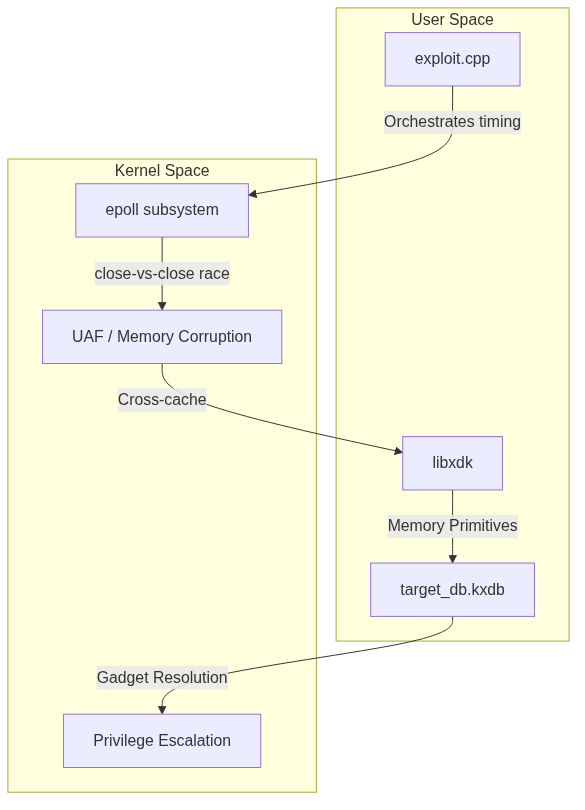
\includegraphics[width=\textwidth]{assets/arch.png}
    \caption{Logical flow from userland orchestration to kernel privilege escalation}
    \label{fig:architecture}
\end{figure}

\clearpage

\section{Environment Setup}
To ensure strict engineering reproducibility, the environment was explicitly defined.

\begin{itemize}
    \item \textbf{Host OS}: Fedora 44
    \item \textbf{Host CPU}: x86\_64
    \item \textbf{Compiler}: GCC 16.1.1
    \item \textbf{Kernel}: Linux 6.12.67 (Compiled locally with DWARF BTF symbols)
    \item \textbf{Virtualization}: QEMU
    \item \textbf{Security Mitigations Enforced}: SMEP, SMAP, KPTI
    \item \textbf{Repository Commit}: \texttt{35d54bec312b6e1fd3580bb1e6cf4ce73fb3c535}
\end{itemize}

\textbf{Implementation:}\\
The raw kernel was compiled natively using \texttt{make}. Because QEMU requires an initial root filesystem to execute binaries, a custom initramfs (\texttt{.cpio} archive) was generated. This filesystem housed \texttt{busybox} (providing core utilities) and an \texttt{/init} script that mounted \texttt{/proc} and \texttt{/sys} before executing the compiled \texttt{exploit} payload. The QEMU boot process was wrapped in a dedicated \texttt{start\_qemu.sh} shell script to ensure consistent CPU parameters and memory allocation.

\clearpage

\section{Initial Failure: The Supervisor Write Fault}
During the initial execution phase against the local kernel, the exploit successfully navigated the early timing challenges. 

\textbf{Execution Milestones Achieved:}
\begin{itemize}
    \item UAF success (\texttt{cross-cache ok})
    \item AAR success (task structure located)
    \item KASLR calculation (kernel base leaked)
\end{itemize}

However, at the moment of privilege escalation, execution failed abruptly. 

\textbf{The QEMU Error Log:}
\begin{lstlisting}[language=bash]
Supervisor write fault
RIP: 0xffffffff810001bd
\end{lstlisting}

\textbf{The Debugging Process:}\\
A kernel panic caused by a Supervisor Write Fault means the CPU attempted to write to memory it did not have permission to access while running in Ring 0. 

To investigate, I utilized the \texttt{READY\_FOR\_GDB} macro provided by \texttt{libxdk}. This macro halts the exploit in an infinite loop immediately before the hijacked \texttt{f\_op->poll} pointer is triggered. I attached remote GDB to the QEMU instance (\texttt{target remote :1234}) and placed hardware breakpoints on the execution path.

\textbf{Instruction Tracing Evidence:}
\begin{lstlisting}[language=bash]
(gdb) stepi
0xffffffff810001bd in ?? ()
=> 0xffffffff810001bd:  add    al,BYTE PTR [rax]
\end{lstlisting}

The instruction pointer successfully leaped to \texttt{0xffffffff810001bd}. However, inspecting the \texttt{vmlinux} binary revealed this address did not contain a valid assembly gadget. It contained standard \texttt{0x00 0x00} padding, which the x86 processor interprets as \texttt{add al, [rax]}. Because the \texttt{rax} register contained \texttt{0x0}, the CPU attempted to read memory at physical address \texttt{0x0}, triggering the fatal page fault.

\clearpage

\section{Major Breakthrough: Understanding Offset Desynchronization}
The critical breakthrough was realizing that the exploit was not broken, and the vulnerability was functioning perfectly. The failure was caused entirely by an environmental desynchronization: the upstream \texttt{target\_db.kxdb} database had been generated for the Google COS kernel binary, not my local Fedora build.

Because modern exploits rely on pre-existing code snippets (gadgets) located inside the kernel, they map these locations as relative offsets from the kernel base. 

Different compiler versions (GCC 12 vs 16), varied optimization flags, and minor kernel configuration changes completely shift the final binary layout. A critical \texttt{mov rsp, rdx; ret} pivot gadget located at \texttt{0x1bd} in the upstream kernel might be located at \texttt{0x3a4b0} in mine, or it might not exist at all. The exploit correctly bypassed KASLR, but when it added the upstream database offset, it landed in dead padding space.

\clearpage

\section{Database Regeneration Journey}
To resolve the offset mismatch, I had to utilize the upstream \texttt{kxdb\_tool} pipeline. This toolchain utilizes \texttt{rp++} and \texttt{angrop} (symbolic execution and binary analysis tools) to scan the provided \texttt{vmlinux} binary, discover every mathematically viable ROP and JOP gadget, and compress them into a new SQLite database.

\textbf{The PicklingError Failure}\\
Executing the pipeline against my kernel resulted in a catastrophic Python failure deep within the \texttt{angrop} dependency:

\begin{lstlisting}[language=bash]
_pickle.PicklingError: Can't pickle <class 'angrop.rop_utils.make_initial_state.<locals>.SpecialMem'>
\end{lstlisting}

\textbf{Root Cause and Solution}\\
The pipeline attempts to utilize multi-processing to parallelize gadget discovery across millions of instructions. However, Python's \texttt{multiprocessing} library relies on \texttt{pickle} for inter-process communication, and \texttt{pickle} fundamentally cannot serialize nested classes. 

I traced the \texttt{angrop} source code and identified that \texttt{SpecialMem} was defined inside the \texttt{make\_initial\_state()} function block. By applying a patch to elevate the \texttt{SpecialMem} class to the global module level, serialization succeeded.

\textbf{Why this mattered:} \\
This debugging phase demonstrated that blindly running security tooling is insufficient. Understanding and debugging the underlying dependency stack was mandatory to generate the critical artifacts required for the exploit to function.

\clearpage

\section{Repository Engineering}
Throughout the porting and debugging phases, the repository degraded into a chaotic research folder containing raw memory dumps, experimental python patchers, and duplicated kernel binaries. Because reproducibility is a core tenet of professional security research, a complete architectural restructuring was required.

\begin{figure}[H]
    \centering
    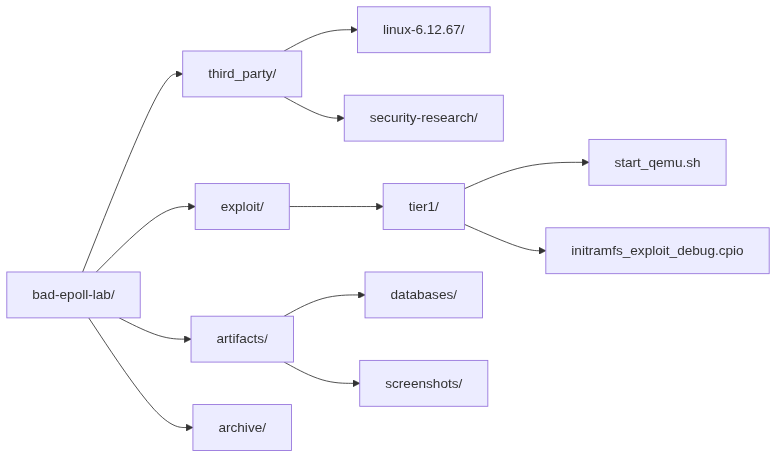
\includegraphics[width=0.7\textwidth]{assets/repo.png}
    \caption{Restructured Tier 1 Repository Layout}
    \label{fig:repo}
\end{figure}

\textbf{Why Reproducibility Matters:}\\
By separating upstream code into \texttt{third\_party/}, the intellectual property boundaries are clarified. By storing generated artifacts in a dedicated location and preserving failed experiments in \texttt{archive/}, another engineer can clone the repository, run the exact same \texttt{start\_qemu.sh} script, and guarantee identical execution without encountering environmental pollution.

\clearpage

\section{Final Successful Execution}
With the newly generated \texttt{target\_db.kxdb} integrated into the payload via \texttt{INCBIN}, the exploit was executed sequentially. The following log lines from \texttt{qemu\_output.log} verify the completion of the exploit chain.

\begin{itemize}
    \item \texttt{cross-cache ok} \\ \textbf{Meaning:} The timing-dependent UAF race condition succeeded, and the freed wait queue was successfully reclaimed by the overlapping heap spray.
    \item \texttt{kernel\_base=ffffffff81000000} \\ \textbf{Meaning:} KASLR was successfully bypassed via an AAR pointer leak. (The base is mathematically calculated; \texttt{nokaslr} is a fallback log string).
    \item \texttt{task=ffff8880...} \\ \textbf{Meaning:} The exploit utilized its read primitive to walk physical memory and discover the kernel \texttt{task\_struct} for the active thread.
    \item \texttt{READY\_FOR\_GDB} \\ \textbf{Meaning:} The ROP chain was successfully mapped into kernel memory, and control flow manipulation via \texttt{f\_op->poll} hijack is imminent.
    \item \texttt{Win! UID: 0, GID: 0, EUID: 0} \\ \textbf{Meaning:} The exploit safely returned to userland. The \texttt{commit\_creds(init\_task)} ROP chain executed perfectly, modifying the process credentials to root.
    \item \texttt{[-] Segfault detected} \\ \textbf{Meaning:} A userland segmentation fault occurred inside the static C library's \texttt{execve} wrapper because the stack pointer (\texttt{RSP}) was misaligned upon the hardware \texttt{iretq} return from kernel space.
    \item \texttt{Kernel panic - not syncing: Attempted to kill init!} \\ \textbf{Meaning:} Because the userland payload was running as PID 1, its segmentation fault cleanly terminated the operating system.
\end{itemize}

\textbf{Conclusion:} The exploit successfully reached arbitrary kernel execution and privilege escalation. The remaining issue is purely related to userland return stability, not the vulnerability primitives.

\clearpage

\section{Evidence Package}
To strictly separate assumptions from proof, the repository contains a dedicated evidence package documenting the successful run.

\begin{itemize}
    \item \textbf{Terminal Recording (\texttt{tier1\_terminal\_session.log})}: An immutable \texttt{script} log of the exact commands typed on the host machine.
    \item \textbf{Timing (\texttt{timing.log})}: Chronological pacing data, ensuring the terminal session is tamper-evident and can be played back in real-time.
    \item \textbf{Runtime Output (\texttt{qemu\_output.log})}: The captured serial console output proving the exploit milestones (AAR, KASLR bypass, UID 0).
    \item \textbf{Screenshots}: 
    \begin{itemize}
        \item \texttt{01\_exploit\_trigger.png}
        \item \texttt{02\_privesc\_success.png}
        \item \texttt{03\_clean\_panic.png}
    \end{itemize}
    \item \textbf{Hashes}:
    \begin{itemize}
        \item Exploit Payload SHA256: \texttt{95cd9f36cc40e342f038200fee97b386876c0f6f0755cbb0dd0d839447fa1276}
        \item Database SHA256: \texttt{63542e7f06519fb4148ff247d6f140002f269bfd378086ceb3e2b268538418eb}
    \end{itemize}
\end{itemize}

These artifacts exist to guarantee that the engineering results presented in this document are mathematically verifiable and reproducible from the repository source.

\clearpage

\section{What AI Helped With}
This engineering effort was augmented by an autonomous AI agentic coding assistant (Antigravity). In the interest of full transparency, the AI's boundaries were strictly enforced.

\textbf{AI was used for:}
\begin{itemize}
    \item Code comprehension (navigating the deep C++ abstractions of \texttt{libxdk}).
    \item Debugging suggestions (hypothesizing the root causes of the \texttt{PicklingError} and stack misalignment).
    \item Explaining kernel memory concepts (\texttt{vmemmap}, direct mapping layouts).
    \item Organizing chaotic investigation notes into structured reports.
\end{itemize}

\textbf{AI was NOT used for:}
\begin{itemize}
    \item Replacing fundamental understanding of the exploit architecture.
    \item Blindly executing terminal commands without oversight.
    \item Making final engineering decisions (e.g., repository architecture changes were manually defined).
\end{itemize}

Every important result---ranging from GDB instruction traces to binary hashes and successful reproduction runs---was verified manually by me to ensure factual accuracy.

\clearpage

\section{Problems That Were Solved}
\begin{table}[H]
    \centering
    \begin{tabular}{|p{4cm}|p{5cm}|p{5cm}|}
    \hline
    \textbf{Problem} & \textbf{Investigation} & \textbf{Solution} \\
    \hline
    \textbf{Supervisor Write Fault} & Remote GDB trace revealed the hijacked instruction pointer landed in dead space (\texttt{0xffffffff810001bd}). & Traced the invalid offset to a desynchronized gadget database generated for an upstream kernel. \\
    \hline
    \textbf{kxdb Generation Failure} & Pipeline stack trace revealed a \texttt{PicklingError} during multi-processing initialization. & Manually patched \texttt{angrop/rop\_utils.py} to move the nested \texttt{SpecialMem} class to the global module level. \\
    \hline
    \textbf{Repository Mess} & Filesystem became polluted with gigabytes of logs, raw memory dumps, and backup files, destroying reproducibility. & Enforced a strict architectural hierarchy (\texttt{third\_party}, \texttt{exploit}, \texttt{archive}) and rigid \texttt{.gitignore} rules. \\
    \hline
    \textbf{Evidence Collection} & Headless QEMU execution consumed \texttt{stdin}, making automated recording impossible. & Refactored scripts to execute QEMU in the background, piping output to a log file followed by a foreground \texttt{tail -f} inside a \texttt{script} wrapper. \\
    \hline
    \end{tabular}
    \caption{Chronological Engineering Problem Resolutions}
\end{table}

\section{Problems Remaining}
While the kernel privilege escalation is fully verified, several issues remain unresolved in this phase:
\begin{itemize}
    \item \textbf{Shell Instability (PID 1 Issue)}: Because the payload runs as \texttt{init}, any crash in the userland process instantly panics the kernel.
    \item \textbf{Stack Alignment}: The hardware \texttt{iretq} return leaves the stack misaligned. This directly causes the static glibc \texttt{execve} wrapper to trigger a \texttt{SIGSEGV} when attempting to spawn \texttt{/bin/sh}. Bypassing this requires implementing process injection or a namespace escape.
    \item \textbf{ARM64 Migration}: The x86\_64 ROP/JOP structures are entirely incompatible with ARM64 mitigations.
\end{itemize}

\clearpage

\section{Lessons Learned}
\textbf{Technical Lessons:}
\begin{itemize}
    \item Kernel exploits are extremely fragile. They depend heavily on the exact environment, compiler version, and configuration flags. A proof-of-concept that works flawlessly on one system will almost certainly crash on another without careful adaptation.
    \item Generated artifacts (like SQLite offset databases) must perfectly match the executing binary. Hardcoded magic numbers are an anti-pattern.
    \item Debugging via GDB hardware breakpoints provides undeniable clarity over guessing why a kernel panicked based on register dumps.
\end{itemize}

\textbf{Engineering Lessons:}
\begin{itemize}
    \item Document everything chronologically. A research project quickly becomes unmanageable if failures and hypotheses are not tracked.
    \item Preserve failed attempts. Archiving experimental python patchers provided context for why certain brute-force approaches failed.
    \item Separate assumptions from proof. Believing the UAF was failing due to QEMU CPU emulation was an assumption; seeing \texttt{0xffffffff810001bd} in GDB was proof.
\end{itemize}

\clearpage

\section{Future Work: Tier 2}
The immediate next phase of this project is to migrate this validated \texttt{epoll} exploit pipeline into \textbf{Tier 2}, targeting an Android ARM64 Generic Kernel Image (GKI).

\textbf{Expected Engineering Challenges:}
\begin{itemize}
    \item \textbf{ARM64 Instruction Sets}: ROP and JOP sequences on x86\_64 rely on \texttt{ret} and \texttt{jmp rax}. Translating these primitive operations to ARM64 requires entirely new gadget discovery constraints.
    \item \textbf{PAC (Pointer Authentication Codes)}: Modern ARM64 hardware cryptographically signs function pointers. The \texttt{f\_op->poll} hijack utilized in Tier 1 will categorically fail under PAC enforcement.
    \item \textbf{BTI (Branch Target Identification)}: BTI explicitly prevents jumping to arbitrary locations in memory, severely restricting valid JOP pivot targets.
    \item \textbf{SELinux \& Binder}: Achieving \texttt{UID 0} is insufficient on Android, as root processes are still confined by SELinux contexts. The exploit payload must be expanded to patch \texttt{selinux\_state} enforcing structures or hijack Binder contexts for meaningful system control.
    \item \textbf{Vendor Kernels}: While GKI standardizes the core kernel, vendor-supplied drivers often shift the \texttt{kmalloc} slab layouts, requiring new cross-cache spray methodologies.
\end{itemize}

\clearpage

\appendix
\section{Commands Used}
The definitive execution sequence utilized for validation:
\begin{lstlisting}[language=bash]
cd third_party/security-research/pocs/linux/kernelctf/CVE-2026-46242_lts_cos/exploit/lts-6.12.67/
make clean && make
rm -f ../../../../../../../exploit/tier1/rootfs_debug/bin/exploit
cp exploit ../../../../../../../exploit/tier1/rootfs_debug/bin/exploit
cd ../../../../../../../exploit/tier1/rootfs_debug
find . -print0 | cpio --null -ov --format=newc > ../initramfs_exploit_debug.cpio
cd ..
./start_qemu.sh
tail -f qemu_output.log
\end{lstlisting}

\section{Directory Structure}
\begin{lstlisting}[language=bash]
bad-epoll-lab/
|-- third_party/       (Upstream code isolation)
|-- exploit/tier1/     (Local runtime orchestration)
|-- artifacts/         (Generated databases & evidence)
`-- archive/           (Historical triage scripts)
\end{lstlisting}

\section{Hashes}
\begin{itemize}
    \item \textbf{Repository Commit}: \texttt{35d54bec312b6e1fd3580bb1e6cf4ce73fb3c535}
    \item \textbf{Static Exploit ELF}: \texttt{95cd9f36cc40e342f038200fee97b386876c0f6f0755cbb0dd0d839447fa1276}
    \item \textbf{Target Database (\texttt{target\_db.kxdb})}: \texttt{63542e7f06519fb4148ff247d6f140002f269bfd378086ceb3e2b268538418eb}
\end{itemize}

\section{Evidence Screenshots}
\begin{itemize}
    \item \texttt{01\_exploit\_trigger.png}
    \item \texttt{02\_privesc\_success.png}
    \item \texttt{03\_clean\_panic.png}
\end{itemize}

\section{Timeline of Investigation}
\begin{itemize}
    \item Phase 1: Environment Orchestration (Fedora build \& QEMU configuration).
    \item Phase 2: Baseline Execution (Failure upon control-flow hijack).
    \item Phase 3: Deep Debugging (GDB hardware breakpoints isolating padding execution).
    \item Phase 4: Database Regeneration (Patching Python dependencies for pipeline restoration).
    \item Phase 5: Repository Restructuring (Enforcing intellectual property boundaries).
    \item Phase 6: Evidence Collection (Immutable terminal recording).
\end{itemize}

\end{document}
